
\documentclass[intern]{cgMA}

\usepackage{csquotes} % Für \enquote
% Dokumentation: https://www.namsu.de/Extra/pakete/Csquotes.html
\usepackage{subcaption} % subfigure/subcaption Umgebungen und \subcaption Befehl
\usepackage{hyperref} % Macht automatisch klickbare Links bei Referenzen etc.
\usepackage{listings} % Für Code-listings o.ä.
\usepackage{graphicx} % Für Graphiken
\usepackage{amsmath,amssymb,amsfonts} % Mathe, Symbole....
\DeclareMathOperator{\Tr}{Tr}
\usepackage{algpseudocode}
\usepackage{algorithm}
\usepackage{float}
\usepackage{gensymb} % Mathe, Symbole....
\usepackage{textcomp} % Symbole....
\usepackage{bm} % \bm{x} Befehl um in Mathe fett zu setzen
\usepackage{cleveref}
\usepackage{blindtext}
\usepackage{titlesec}
\nocite{*}
\usepackage[
    backend=biber,
    style=ieee,
    dashed=false,
    sortlocale=en_US,
    natbib=true,
    url=true, 
    doi=true,
    eprint=false
]{biblatex}
\addbibresource{sources.bib}

\title{Real-time Simulation of Granular Matter using Smoothed Particle Hydrodynamics}
\author{André Neder}
\zweitgutachter{Alexander Maximilian Nilles, M.Sc.}
\zweitgutachterInfo{(Institut für Computervisualistik, AG Computergraphik)}
% \externLogo{7.46cm}{logos/ExternLogoPlaceholder}
% \externName{DIN: NewTechnologies}

\begin{document}
    \maketitle
    \newpage
    \tableofcontents
    \newpage
    \pagenumbering{arabic}
    \section{Introduction}

    Granular matter consists of discrete, macroscopic particles that interact through contact forces, exhibiting unique behaviors such as flowing, layering or piling. Simulating such behaviors in realistic scenarios is especially challenging, due to the necessity of employing a very high number of discrete elements to achieve visually plausible simulations. Granular materials find diverse applications across geophysics, civil engineering, pharmaceuticals, and other industries, playing crucial roles in phenomena such as landslides, construction, powder mixing, storage and transportation. A powerful technique for simulating such materials is Smoothed Particle Hydrodynamics (SPH). SPH is a meshless Lagrangian method that has been employed a lot in fluid dynamics and can also be used to simulate granular behavior. By combining well-established SPH techniques for simulating granular materials with the latest developments in SPH research, real-time simulations might become achievable. In the pages ahead, I will assess the doability of real-time simulations for granular matter, by combining established methods and recent advancements to achieve a dynamic and interactive implementation.
    \pagebreak
    \section{Related Work}
    \dots
    \pagebreak
    
    \section{Basics}

    \subsection{Navier-Stokes equation}
    The basic concept behind most fluid simulations lies in the Navier-Stokes equations, which describe the motion of fluids and deformable solids. As granular flow can be interpreted as a kind of fluid they will be employed here aswell. One of the most important parts is the continuity of mass equation, which \enquote{describes the evolution of an object's mass density $\rho$ over time, i.e.,} \cite{survey_on_sph}
    
    \begin{equation}
        \frac{D \rho}{D t} = -\rho(\nabla v)
    \end{equation}

    with $v$ beeing the velocity and $\nabla$ the gradient operator. It states that the mass of fluid entering a given region must be equal to the mass leaving that region, accounting for any change in density within the fluid. The second part is the incompressible Navier-Stokes equation

    \begin{equation}
        \rho \frac{D v}{D t} = -\nabla p + \mu \nabla^2 v + f_{ext}
    \end{equation}

    which describes the conservation of momentum. Here \enquote{the pressure $p$ can be interpreted as a Lagrange multiplier that has to be chosen such that the}\cite{survey_on_sph} conservation of mass is fulfilled. $\mu$ denotes the dynamic viscosity of the fluid and $f_{ext}$ the influence of external forces.

    \subsection{Signed Distance Functions}
    Signed distance functions (SDF) are a versatile tool in computer graphics. They determine the shorted distance of a point in space to the surface of geometric object, while preserving information about if the point is inside or outside the object. This allows for precise implicit reconstruction of surfaces. A greate source for understanding and utilizing SDFs has been \cite{iquilezles}. 

    \begin{figure}[H]
            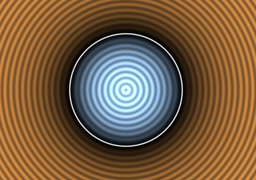
\includegraphics[width=0.5\textwidth]{figures/gfx00.png}
            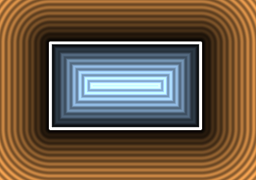
\includegraphics[width=0.5\textwidth]{figures/gfx02.png}
        \caption{SDF of a circle and a box in 2D \cite{iquilezles2}}
    \end{figure}

    \subsection{Bitonic Sort}

    Bitonic merge sort is a sorting algorithm with a performance complexity of $O(\log^2(n))$. The algorithm can be implmented on the GPU to achieve a massive performance increase by parallelization. In this work, a modified version of the implementation by \href{https://twitter.com/tgfrerer}{@tgfrerer} has been used \cite{bitonic}. The algorithm uses a pattern of comparison to sort a list of elements in parallel. The algorithm has been modified to use Vulkan's Push Constants to select the type of comparison inside of the shader provided by \cite{bitonic}. Another change is the use of Specialization Constants to set the local workgroup size of the compute shader invocation.

    \begin{figure}[H]
        \begin{center}
            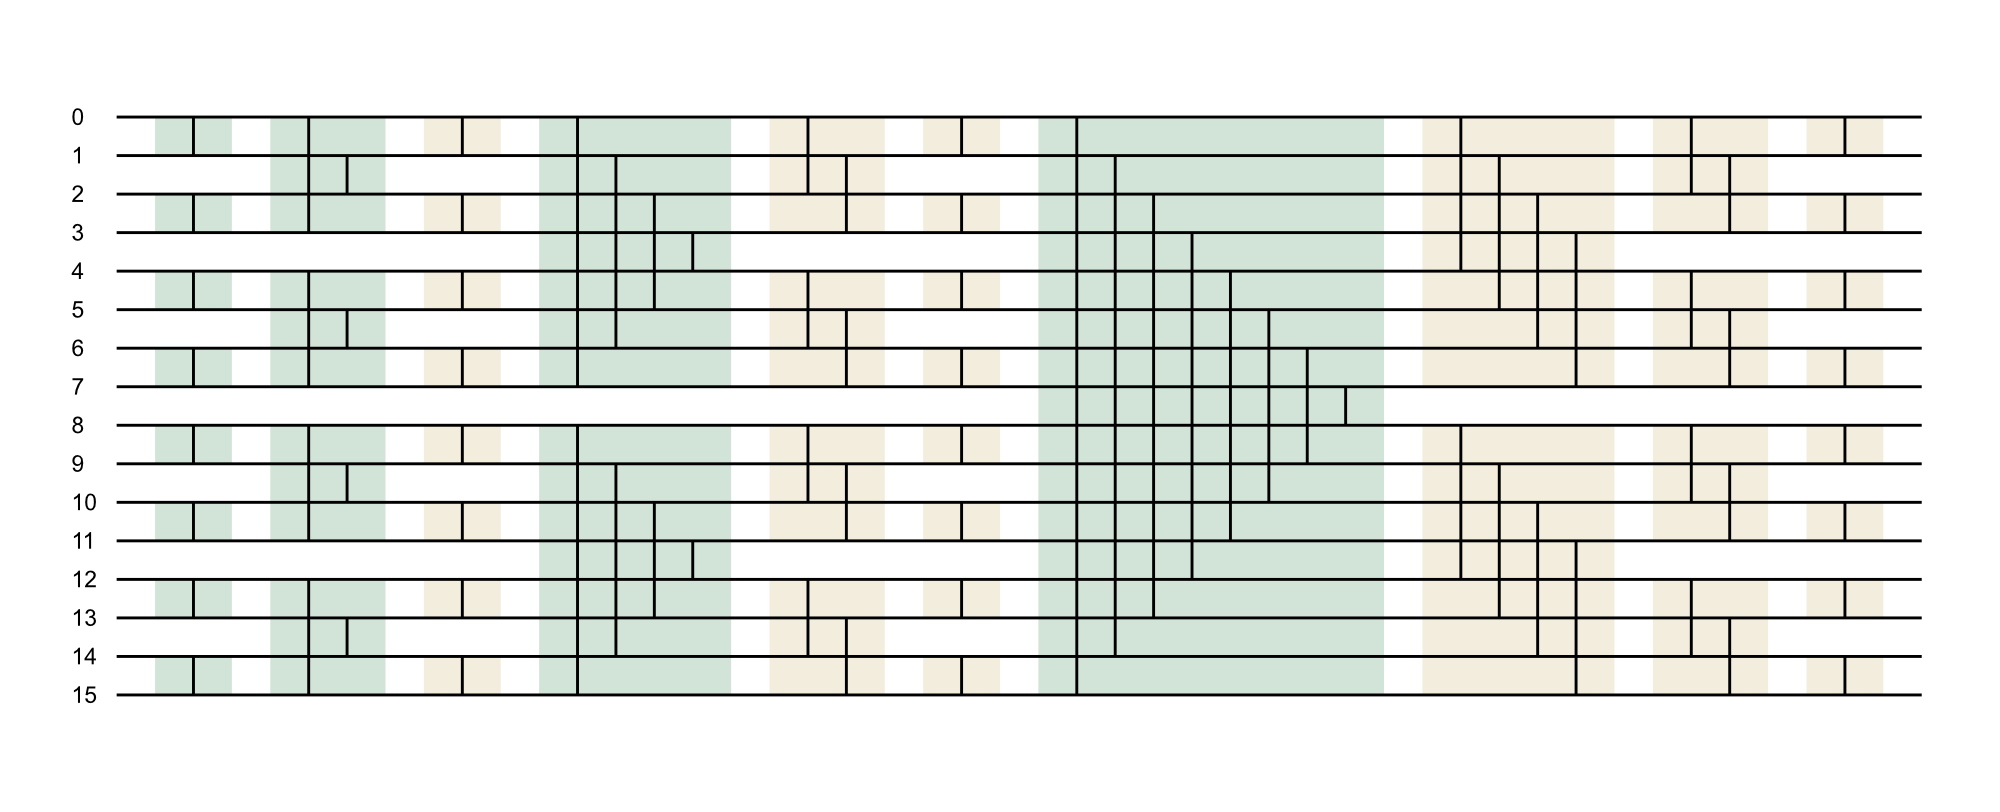
\includegraphics[width=1\textwidth]{figures/bitonic_sort.png}
        \end{center}
        \caption{Sorting diagram for 16 sortable elements. Horizontal lines represent array indices into our array of sortable elements, each vertical line represents one worker thread performing a compare-and-swap operation. \cite{bitonic}}
    \end{figure}

    \pagebreak
    \section{Method}
    \subsection{Smoothed Particle Hydrodynamics}
    Smoothed Particle Hydrodynamics (SPH) is a computational technique widely employed in fluid dynamics and other fields for simulating complex physical phenomena.SPH represents the fluid or material as a collection of discrete particles. Each particle has physical properties such as density, pressure and velocity. 

    These interact through a kernel function $W$ with radius $h$, which smoothes these properties over neighboring particles, allowing for a continuous representation of the material and facilitating the simulation of intricate behaviors, including fluid flow, collisions, and deformations. An arbitrary field $A$ can be approximated as shown, with an error in the order of $h^2$.

    \begin{equation}
        A(r) \approx \int A(r') W(|r - r'|, h) d(r')
    \end{equation}
    
    The integral is then approximated using a Riemann summation over the neighboring particles.

    \begin{equation}
        A(r) \approx \sum_j A_j W(|r - r_j|, h)
    \end{equation}

    This concept is then applied to calculate the properties of a given particle. SPH's versatility extends beyond fluids, making it applicable to problems involving granular materials, astrophysics, and even solid mechanics. 

    //Todo: more about the kernel ?

    \subsubsection{Weakly Compressible SPH}
    Weakly Compressible Smoothed Particle Hydrodynamics (WCSPH) is a variant of the traditional SPH method where, the incompressibility constraint is relaxed, allowing for a more computationally efficient simulation while still capturing the essential fluid behaviors. This approach is particularly useful in scenarios where the fully incompressible SPH formulation might be computationally expensive and it finds a sweet spot between precision and computational efficiency.This is especially usefull in the context of large-scale simulations or real-time applications.

    \subsubsection{Predictive-Corrective Incompressble SPH} 
    Predictive-Corrective Incompressible Smoothed Particle Hydrodynamics (PCISPH) is an advancement in the SPH method designed to address issues related to incompressibility in fluid simulations. It employs a two-step process where a predictive step estimates particle velocities and a corrective step which iteratively adjusts these velocities to enforce incompressibility. This technique is particularly useful in scenarios where traditional SPH methods such as WCSPH struggle with maintaining fluid volume conservation, providing more accurate and stable simulations, especially for scenarios involving complex fluid interactions, like fluid splashes or turbulent flows.

    \subsubsection{Implicity Incompressble SPH}
    Implicit Incompressible Smoothed Particle Hydrodynamics (IISPH) is a variant of the SPH method that also addresses the challenge of maintaining incompressibility in fluid simulations. Unlike traditional SPH methods, IISPH employs an implicit formulation for the pressure term in the Navier-Stokes equations, allowing for larger time steps and improved stability. %This method is particularly useful in simulating incompressible fluid flows where maintaining constant density is essential, providing a more efficient and stable approach compared to explicit methods in certain scenarios, such as large-scale simulations or real-time applications.%

        
    \subsection{Libraries \& Technologies}

    \subsubsection*{C++ \& Vulkan}
    When choosing a framework for a fluid simulation using SPH most papers use C++ in combination with OpenMP to achieve parallelization, other implementations involve Cuda to use the massive parallel compute performance of GPUs.(SRC) For rendering these simulations, dedicated renderers are used. In this implementation Vulkan is used to simulate and visualize the granular material on the GPU using a combination of compute shaders and the rasterization pipeline. This allows for massive parallel computation of the simulation togehter with the visualization in real time, giving maximum flexibility and extensibility by for example a raytraced visualisation. Vulkan uses SPIRV Shaders, which allows the use of any shading language, that can be compiled to it. I opted for GLSL for its well known C like structure. \url{https://www.vulkan.org/}

    \subsubsection*{CMake}    
    CMake is a popular choice in software development for its role as a cross-platform build system and project configuration tool, streamlining the build process, enhancing code portability, and offering flexibility in managing diverse project structures and dependencies. \url{https://cmake.org/}

    \subsubsection*{Vulkan Memory Allocator}   
    In difference to other Graphics APIs Vulkan requires the programmer to do the memory management on the GPU. Vulkan Memory Allocator (VMA) is employed to achive efficient management and optimization of GPU memory, simplifying memory allocation and deallocation processes and improving overall performance. \url{https://gpuopen.com/vulkan-memory-allocator/}

    \subsubsection*{shaderc}   
    Shaderc is utilized for the compilation and linking of shaders due to its user-friendly interface and simplicity in handling these processes. This made is straight foward to compile the used GLSL shaders to SPIRV for Vulkan to use. \url{https://github.com/google/shaderc}

    \subsubsection*{TinyGLTF \& STB Image}  
    In computer graphics, TinyGLTF is often used for seamless glTF asset loading, and STB Image is favored for its straightforward approach to handling and processing images, both known for their efficiency and ease of use across different applications. \url{https://github.com/syoyo/tinygltf}

    \subsubsection*{Dear ImGui}
    Dear ImGui is a popular immediate mode graphical user interface (GUI) library. It simplifies the process of creating and integrating user interfaces into applications by providing an intuitive and efficient framework and has implementations for nearly every common graphics API and windowing library. It also supports features like multiple viewports and docking elements to them. \url{https://github.com/ocornut/imgui}

    \subsubsection*{GLFW}
    GLFW is a widely-used windowing library that simplifies the creation and management of windows, handling user input and facilitating cross-platform development for OpenGL- and Vulkan-based applications. \url{https://www.glfw.org/}

    \subsubsection*{glm}
    GLM is a versatile C++ mathematics library designed for graphics programming, providing a comprehensive set of functions and classes for vector and matrix operations commonly used in computer graphics. \url{https://github.com/g-truc/glm}

    \subsubsection*{TriangleMeshDistance}
    TriangleMeshDistance offers a user-friendly programming interface for effortlessly creating signed distance fields of adjustible resolution from 3D meshes. \url{https://github.com/InteractiveComputerGraphics/TriangleMeshDistance}

    \pagebreak
    \section{Implementation}
    \dots
    
    \begin{algorithm}
        \caption{Full Simulation Frame}
        \begin{algorithmic}[1]
        \State find neighbors 
        \State compute $\rho$ and $F^{drag}$ 
        \State compute $s$ 
        \State compute $v$ advection 
        \State compute $\rho$ advection 
        \State $l = 0$
        \While {$l < 2$ $||$ $\rho_{avg} - \rho_0 < \eta $}
            \State compute $d_{ij}p_{j}$
            \State compute $p^{l+1}$
            \State $p(t) = p^{l+1}$
            \State apply yield criterion 
            \State $l = l+1$
        \EndWhile
        \State compute $F^p$ and $F^f$ 
        \State integrate 
        \State advect HR particles 
        \end{algorithmic}
    \end{algorithm}

    \subsection{Neighborhood Search}
    Using the SPH approximation involves finding all neighboring particles within the smooting length $h$. In a naive implamentation this means iterating all other particles and check their distance to each other. With a runntime of $O(n^2)$ this is not an option for a realtime scenario. To improve the neighborhood search a number of algorithms could be employed. In this implementation a grid based approach has been used, where every particle is first segmented into a spatial grid with cell size of $h$. This provides the possibility to find every neighbor of a given particle, by finding its cell and iterating over its members and all adjacent cells. This dramatically decreses the amount of particles that have to be checked every frame. To get a list of particles for each cell, all grid entries, consisting of a cell key and a particle ID, are first sorted by the cell key. As this sorting has to be done at the beginning of every frame, this has to be done as fast as possible. To achive this, a parallel sorting algorithm, such as radix sort or in this case bitonic merge sort is used. After the list of grid entries has been sorted, the start of every cells entries has to be found, by checking if the cell key of an entry and its predecessor are the same. The starting index of the cell is then stored in an array of length of $n$, being the particle count, at the position of the cellkey. This implies that all cell keys have to be within the range $0$ to $(n - 1)$. 
    When iterating over a given cells entries, the entries particle ID is used to check if the particle is within the smoothing length. A cell is found by calculating a particles cell key an the keys of its neighboring cells, and looking up the starting index of that cells entries. The entries can then be iterated until the cell key changes. In the below examples a list of 8 grid entries is shown, first in their unsorted state, then after they have been sorted and lastly the list of starting indices of each cell, where $-1$ denotes entries where no cell starts. In the actual implementation unsigned integers are used to represent the starting indices and the maximum unsigned integer is used for empty cells. 
    
    \begin{table}[ht]
        \centering
        \caption{Example of unsorted list of grid entries }
        \begin{tabular}{ l c c c c c c c c }
            Cell key    & 2 & 7 & 5 & 3 & 7 & 7 & 5 & 2 \\ 
            Particle ID & 0 & 1 & 2 & 3 & 4 & 5 & 6 & 7 \\   
        \end{tabular}
    \end{table}

    \begin{table}[ht]
        \centering
        \caption{Example of sorted list of grid entries }
        \begin{tabular}{ l c c c c c c c c }
            Cell key    & 2 & 2 & 3 & 5 & 5 & 7 & 7 & 7 \\ 
            Particle ID & 0 & 7 & 3 & 2 & 6 & 1 & 4 & 5 \\   
        \end{tabular}
    \end{table}

    \begin{table}[ht]
        \centering
        \caption{Example of list of starting indices }
        \begin{tabular}{ l c c c c c c c c }
            Starting indices    & -1 & -1 & 0 & 2 & -1 & 3 & -1 & 4 \\ 
        \end{tabular}
    \end{table}

    This approach allows the grid to have an undefined size as only the amount of particles matters for the creation of it. 

    \subsection{Density}  
    When implementing a SPH simulation the first thing to do is calculate the density $\rho$ of a particle. It is determined by a sum over the neighboring particles. The volume $V$ of each particle within the smoothing length $h$ is multiplied with the density of it and the weighting kernel $ W_{ij} \equiv W(x_i - x_j, h)$. As the volume can be expressed as $V = \frac{m}{\rho}$ we can simplify the equation to only the sum of weighted masses. (SRC)

    \begin{equation}
        \rho_i = \sum_j V_j \rho_j W_{ij}
        = \sum_j m_j W_{ij}
    \end{equation}

    \subsection{Unilateral incompressibility}  
    The next step of the simulation is to compute a pressure that compensates the difference in density between particles. The density and pressure underlie the principle of unilaterial incompressibility, which can be expressed in the form: 
    \begin{equation}
        \rho_i \leq \rho_0 \; \bot \;  p \geq 0
    \end{equation}
    This says that the density of a given particle $i$ can not be greater than the rest density of the material and the pressure can not become negative.

    \subsection{External forces}
    A change in density can be achived by applying external forces to the particles. 
    \subsection{Gravity}
    Gravity is given as a fixed acceleration in a given direction in 3D space. Multiplied with the weight of a given particle we get an actual force.
    \subsection{Drag}
    As an additional force that approximated the interaction with air a drag force $F^{drag}$ was applied. Which uses a simplified implementation of the drag by (SRC). For this the relative velocity difference of a particle to the surrounding air is computed and its length squared. (SRC)

    \begin{equation}
        v^2_{i,rel} = |v_a - v_i|^2\ \frac{v_a - v_i}{|v_a - v_i|}
    \end{equation}

    The velocity of the air $v_a$ can be set to 0 or could be taken from a velocity field of some kind. Computing the drag force, to apply to each particle, involves determining the crosssecional area $A_i$ of a particle. This can be represented by the area of a circle. Then the actual area exposed to oncomming air needs to be determined. For this a cone which is defined by the direction of the relative velocity differnce and a set angle is used to check if there are any other particles that shield the current particle form the air. This is done by a dot product of the relative velocity difference and the vector to the neighboring particles, which returns the angle between them. To not only get a boolean value for the shielding, an occlusion value is introduced, which is set to the smallest angle between neighboring particles in the cone. This value is then subtracted from 1 and added to the drag formulation as weight $\omega$. Further parameters for the equation are $\rho_a$ the density of the air or the medium that surrounds the particles and $C_{D,i}$ the drag coefficient for shape of the particle. The whole formula is then composed as: 

    \begin{equation}
        F^{drag}_i = \frac{1}{2}\rho_a v^2_{i,rel} C_{D,i}  \omega  A_i
    \end{equation}

    The deformation of a particle by the surrounding air is left out in this implementation.

    \subsection{Strain \& Stress}
    
    To simulate friction between the particles of the granular material we first need to calculate the strain $\varepsilon$, which measures the deformation of a material under external forces and is represented as a tensor of rank 3. This involves determining the velocity gradient $\nabla u_i$ by an outer product with the kernel gradient $\nabla W_{ij}$. 
    
    \begin{equation}
        \nabla u_i = \sum_j V_j \nabla W_{ij} u_j^T
    \end{equation}

    The strain is then computed as:
    \begin{equation}
        \varepsilon = \frac{1}{2} (\nabla u_i + \nabla u_i^T)
    \end{equation}

    What is stress...
    For the computation of the frictional stress a parameter $D$, which relates the frictional stress $s$ to the dissipation of strain, is calculated as:

    \begin{equation}
        D_i = \frac{2 m_i^2 \Delta t}{\rho_i^2} \sum_j \frac{1}{\rho_j} \nabla W_{ij}  \nabla W_{ij}^T
    \end{equation}
    % $\nabla W_{ij}  \nabla W_{ij}^T \equiv W_{ij} \otimes W_{ij}$\\
    The paramter can be precomputed for a prototype particle with a filled neighborhood, to make the compution more efficient.
    The stress is obtained by multiplying the strain tensor with the inverse of $D$. 
    
    \begin{equation}
        s_i = D^{-1} \varepsilon
    \end{equation}

    For most dry granular materials there is no or neglectable cohesion (The tendency of particles to stick to each other). This means that we can subtract the mean hydrostatic stress $s_{i, hydrostatic}$ from the stress computed above, enforcing a traceless deviatoric stress $s_{i, deviatoric}$, which will further be used as $s_i$. 

    \begin{equation}
        s_{i, hydrostatic} = \frac{1}{2} \Tr s_i 
    \end{equation}
    \begin{equation}
        s_{i, deviatoric} = s_i - s_{i, hydrostatic} 
    \end{equation}

    Cohesion can be handled similarly to friction. (...)

    The amount of friction that can be applied is limited by the pressure. This is expressed by the Drucker-Prager yield criterion:

    \begin{equation}
        ||s_i|| \leq p_i \alpha
    \end{equation}

    \begin{equation}
        \alpha = \sqrt{2} \sin \Theta
    \end{equation}

    where $\alpha$ is the frictional coefficient for an angle of repose $\theta$ (the maximum angle a material can pile before slipping) and $||s_i||$ the frobenius norm of $s_i$.The yield constraint can be approximated in a piecewise linear manner by applying it to each component of $s$

    \subsection{Pressure}
    In traditional SPH methods the pressure $p$ is calculated by an equation of state like the ideal gas equation
    \begin{equation}
        p_i = k * (\rho_i - \rho_0)
    \end{equation}
    or Tait's equation 
    \begin{equation}
        p_i = \frac{\rho_0 * B}{n} n \frac{\rho_i}{\rho_0}^n
    \end{equation}
    where $k$, $B$ and $n$ are parameters controlling the stiffness of the pressure calculation, which means the scaling of a density error and the resulting pressure.
    PCISPH then tries to minimize the mean density error by doing multiple iterations, correcting the pressure to apply. As WCSPH does not provide a good enough incompressibility for stable friction calculations and PCISPH can take a lot of iterations to converge, I opted for IISPH as it provides pressures that result in a very small mean density error, after only few iterations and supports larger timesteps as other variants of SPH.

    The IISPH implemetation consist of two parts. The first being the advection of the velocities and densities and the second, the iterations to solve for the pressure. For the advection all external forces are summed up and the particle velocities are advanced in time to get an intermediate velocity $v_i^{adv}$. \cite{6570475}

    \begin{equation}
        F_i^{adv} = F^g + F_i^{drag}
    \end{equation}

    \begin{equation}
        v_i^{adv} = v_i + \Delta t \frac{F_i^{adv}}{m_i}
    \end{equation}

    The intermediate velocity is then used to calculate predicted densities $\rho_i^{adv}$ for all particles. \cite{6570475}

    \begin{equation}
        \rho_i^{adv} = \rho_i + \Delta t \sum_j m_j v_{ij}^{adv} \nabla W_{ij}
    \end{equation}
    // TODO: Pressure calculation
    pressure
    \begin{equation}
        p_i^{l+1} = (1 - \omega) p_i^l + \omega \frac{1}{a_{ii} * \Delta t^2} (\rho_0 - \rho_i^{adv} - \Delta t^2 \psi)
    \end{equation}
    $\omega = 0.5$
    \begin{equation}
        \psi = \sum_j m_j (\sum_j d_{ij}p_j^l - d_{jj}p_j^l - \sum_{k \neq i} d_{jk}p_k^l) \nabla W_{ij}
    \end{equation}
    \begin{equation}
        \sum_{k \neq i} d_{jk}p_k^l = \sum_{k} d_{jk}p_k^l - d_{ji}p_i^l
    \end{equation}
    \begin{equation}
        \rho_i^{l+1} = |p * a_{ii} * \Delta t^2 - (\rho_0 - \rho_i^{adv} - \Delta t^2 \psi)| + \rho_0
    \end{equation}

    \begin{equation}
        a_{ii} = \sum_j m_j (d_{ii} - d_{ji}) \nabla W_{ij}
    \end{equation}

    \subsection{Internal Forces}
    
    For the calculation of the pressure force of a given particle the SPH concept is applied. 

    \begin{equation}
        F_i^p = -m_i \sum_{j \neq i} m_j (\frac{p_i}{\rho_i^2} + \frac{p_j}{\rho_j^2})  \nabla W_{ij}
    \end{equation}
    
    A similar formulation can be used to determine the frictional force of that particle.

    \begin{equation}
        F_i^f = -m_i \sum_{j \neq i} m_j (\frac{s_i}{\rho_i^2} + \frac{s_j}{\rho_j^2})  \nabla W_{ij}
    \end{equation}

    

    \subsection{Integration}
    For the integration of the simulation a simple Euler integration has been used. It could be exchanged for a more advanced integrations scheme such as Leap-Frog or Verlet.
    \begin{equation}
        v_i(t + \Delta t) = v_i^{adv} + \Delta t \frac{F_i^p}{m_i}
    \end{equation}
    \begin{equation}
        x_i(t + \Delta t) = x_i + \Delta t v_i(t + \Delta t)
    \end{equation}

    \subsection{Boundary Handling}
    
    \subsubsection{Particle-Based Approaches}
    Most implementations of SPH use the concept of AK et al. when implementing boundary handling and rigidbody interactions. The idea is to represent boundaries and rigidbodys by sampling their surface or volume with a dense mesh of particles, which can then be incoporated into the normal simulation. For static objects the boundary particles are not integrated in time. For dynamic rigidbodies the particles representing them, collect the counteracting forces, they excert onto the fluid. The collected forces can then be integrated by a rigidbody physics solver.
    This method presents some drawbacks. One of them being the amount of particles required to sample the 3D models in the scene, which then have to be checked for each neighboring fluid particle.

    \subsubsection{Volume Maps}
    In this implementation the concept of Volume Maps is employed. They are an implicit boundary representation, inspired by the density maps concept. They use signed distance functions to determine the volume of the intersection of the kernel function around a particle and the boundary. For this, the boundary or bounding box of any arbitrary mesh is extended by the kernel radius and then sampled on a grid with a set resolution. Here the TriangleMeshDistance library is used to create a signed distance representation of any triangle based mesh. For each sample a vector to the nearest point on the surface of the object is stored aswell as the intersection volume $V_B$, which is calculated by the signed distance $\Phi$, treated by a cubic extension function $\gamma^*$, to get a continuos differentiable function, which results in a smooth transition at $x = h$. \cite{10.1145/3359566.3360077}

    \begin{equation}
        V_b(x) = \int_{N(x)}\gamma^*(\Phi(x'))dx'
    \end{equation}

    \begin{equation}
        \gamma^*(x) = 
        \begin{cases}
            \frac{C(x)}{C(0)},& \text{if } 0 < x < h \\
            1,& \text{if } x \leq 0 \\
            0,              & \text{otherwise}
        \end{cases}
    \end{equation}

    For this cubic extension function the cubic spline kernel $C(x)$ \cite{doi:10.1146/annurev.aa.30.090192.002551} is used. The use of this function does not enforce the use of the same function for the SPH approximation, where any kind of kernel function can be used. \cite{10.1145/3359566.3360077}
    The grid is then stored as a 32-bit 4-channel floating point 3-dimensional image and uploaded to the GPU. As Vulkan does not support arrays of 3D images, as it does for 2D, the descriptor indexing extension has to be used to allow for multiple 3D textures being bound dynamically. When sampling the texture in the shader, the nearest position on the surface and the intersection volume can be determined using only one texture read access instead of iterating all neighboring boundary particles as done in the particle-based approach. After transforming the volume map from its texture space into world space inside of the shader, a smooth value for both required properties is can be determined by the sampler. These values can the be used in any of the above mentioned equations, by subsituting the mass for the determined volume $V_b$ and the reference density of the simulated material $\rho_0$.

    \begin{equation}
        \rho_i = \sum_b V_b \rho_0 W_{ib}
    \end{equation}

    \begin{equation}
        F_i^f = -m_i \sum_{b} V_b \rho_0 (\frac{s_i}{\rho_i^2}) \nabla W_{ib}
    \end{equation}
    \begin{equation}
        F_i^p = -m_i \sum_{b} V_b \rho_0 (\frac{p_i}{\rho_i^2}) \nabla W_{ib}
    \end{equation}

    For the calculation of the resulting boundary forces only the pressure and stress of the particle is used, other than in the calculation of the forces between particles, where both particles contribute to the force. At this point the boundary forces can be applied to the actual rigidbody the volume map represents, to allow for two way coupling of the simulation and the boundaries.

    \subsection{Upsampling}
    As granular matter consists of vast number of grains, simulating them all as individual particles, would not only make the computational cost and memory consuption incredibly high, but would also result in a very restricted time step due to the CFL condition. To achive real time results, the simulation is done for a set of low-resolution (LR) particles which approximate the granular flow, which are then upsampled to another set of high-resolution (HR) particles. \cite{10.2312:PE:vriphys:vriphys12:053-060}
    % The volume of each low-resolution particle is initially sampled with a special pattern of high-resolution particles, which tries to minimize the effect of clumping. For this pattern, 
    \\// TODO: Sampling

    After the above described algorithm is executed on the low-resoltion particles, the high resolution particles are advected based on the velocity field of the low-resolution simulation. This is again done by the SPH concept, but with a different smoothing length $h_{HR}$ which is set to $h_{HR} = 3h_{LR}$. To find the velocity of a HR particle a distance based weight $w$ is introduced.

    \begin{equation}
        w(d_{ij}) = \max(0, (1 - \frac{d_{ij}^2}{h_{HR}^2})^3)
    \end{equation}

    In this equation $i$ refers to a high-resolution particle and $j$ to a low-resoltion particle or a boundary and $d_{ij}$ to the distance between them. The velocity is the computed as the weighted average velocity over the neighboring LR particles.\cite{10.2312:PE:vriphys:vriphys12:053-060}

    \begin{equation}
        v_i^*(t + \Delta t) = \frac{1}{\sum_j w(d_{ij})}\sum_j w(d_{ij})v_j
    \end{equation}

    As the LR particles should be able to not only follow the flow of the granular material, but react to gravity when there are no LR particles in its range, a blending weight $\alpha$ is introduced, to define the contributions of the simulation and external forces. The final velocity of each HR particle is then computed as:

    \begin{equation}
        v_i(t + \Delta t)  = (1 - \alpha)v_i^*(t + \Delta t) + \alpha(v(t) + \Delta t \frac{F^g}{m})
    \end{equation}

    where $\alpha$ is:

    \begin{equation}
        \alpha = 
        \begin{cases}
            1 - \arg \max_j w(d_{ij}),& \text{if } \frac{\arg \max_j w(d_{ij})}{\sum_j w(d_{ij})} \geq 0.6 \\
            1 - \arg \max_j w(d_{ij}),& \text{if } \arg \max_j w(d_{ij}) \leq w(r_{LR}) \\
            0,              & \text{otherwise}
        \end{cases}
    \end{equation}

    The constant $0.6$ is an empirically tested value for the above defined high-resolution smoothing length. \cite{10.2312:PE:vriphys:vriphys12:053-060}
    
    \subsection{Visualization}
    \dots
    \pagebreak
    \section{Evaluation}
    \dots
    
    \subsection{Performance}
    \dots
    \pagebreak
    \section{Conclusion \& Future Work}
    \dots
    
    \pagebreak
    \printbibliography
\end{document}